\documentclass{article}

\usepackage[utf8]{inputenc}
\usepackage{xcolor}
\usepackage{textcomp}
\usepackage[T1]{fontenc}
\usepackage{pdfpages}

\title{deutsch}
\author{marius cramer}
\date{15-08-2018}

\definecolor{myGreen}{RGB}{97, 154, 76}
\definecolor{myRed}{RGB}{176, 72, 72}
\definecolor{myBlue}{RGB}{77, 130, 185}
\definecolor{myOrange}{RGB}{221, 137, 51}

\begin{document}
\maketitle

\tableofcontents

\newpage

\section{Bewertung Leseabend}
\begin{enumerate}
  \item Raumgestaltung (max. 6 Punkte)
  \item Lesekompetenz/Kommunikationsleistung (max. 15 Punkte)
  \begin{itemize}
    \item flüssiges; sinngestaltendes Lesen
    \item Präsentationsleistung
    \item Zuhörerbezug
  \end{itemize}
  \item Methodischer Ablauf/Konzeption (max. 6 Punkte)
\end{enumerate}

\section{Assoziation}
Zum Wort Träume:
\begin{itemize}
  \item Schlaf
  \item Gedanken
  \item Denken
  \item imaginär
  \item fiktiv
  \item Wunsch
  \item ideal
  \item perfekt
  \item Ausweg
  \item bunt
\end{itemize}

\medskip

\medskip

zum Weitergehen eines Hörspiels:
\begin{itemize}
  \item illegaler Generator, zum Unterbringen von Flüchtlingen
  \item Mutter findet nach Entdeckungssuche heraus was das Geräusch erzeugt und ist shockiert.
\end{itemize}

\section{Literatur}
Aufbau eines klassischen Dramas:
\begin{enumerate}
  \item Exposition
  \begin{itemize}
    \item Einführung in Ort, Zeit, Person und Handlung
    \item Andeutung des Konfliktes
  \end{itemize}
  \item Ansteigen der Handlung/erregendes Moment
  \begin{itemize}
    \item Handlungsfäden werden verknüpft
    \item Intrigen werden gesponnen
    \item Entwicklung des Geschehens geht in eine Richtung
  \end{itemize}
  \item Höhepunkt und Peripetie
  \begin{itemize}
    \item Höhepunkt u. Peripetie
    \item Konflikt gelangt zum Höhepunkt
    \item Held / Helden stehen vor der entscheidenden Auseinandersetzung
    \item Peripetie -\guilsinglright Umschlag zur dramatischen Wende zum Sieg oder Niederlage
  \end{itemize}
  \item Fallende Handlung mit retardierenden Moment (Moment der letzten Spannung)
  \begin{itemize}
    \item 'Wird der Held noch mal gerettet?'
  \end{itemize}
  \item Katastrophe
  \begin{itemize}
    \item Lösung des Konfliktes (Tragödie -\guilsinglright Untergang des Helden)
  \end{itemize}
\end{enumerate}

\section{Aufgaben zum Inhalt von "Träumen" (Der fünfte Traum)}
Welche Informationen über Ort, Zeit und Handlung haben sie dem Hörspiel entnommen?
\begin{itemize}
  \item Ort: Lucy's Wohnung in New York
  \item Zeit: Nachmittag, ungefähr 16:30
  \item Handlung: Mutter besucht Lucy in neuer Wohnung und freut sich diese endlich zu sehen. Darauf hin wundert sie sich was das 'merkwürdige' Geräusch im Hintergrund ist. Lucy wimmelt ab und sagt es wäre der Lift. Danach macht Lucy das Radio an und Lucy geht in die Küche. Die Mutter sieht nach dem Fahrstuhl, denn sie hört ihn auch mit laufendem Radio. Sie entdeckt das der Lift gar nicht aktiv ist, das Geräusch ist trotzdem da. Lucy wird ganz nervös und schlägt vor die Mutter ginge ins Wohnzimmer zurück. Als sie zurück kommt, läuft im Radio ein Vortrag über Termiten. Lucy kommt ins Zimmer gerannt und die Mutter kommt darauf, dass das Geräusch von den Termiten entstammt. Dann wird die Mutter müde und stirbt. Kurz nach 17:30 kommt Bill nach Hause und stirbt auch.
\end{itemize}

\par

Hörspiel "Träume"  Günther Eich
\begin{itemize}
  \item eines der bedeutendsten Hörpsiele der 50er Jahre des 20. Jahrhunderts
  \item 5 Einzelträume -\guilsinglright Alpträume
  \item Schauplatz der Handlung jeweils anderer Erdeteil
  \item Traumszenen zwischen 1947-1950
  \item nachEichs Notizen: Datum des leztzten Traums: 31. August 1950
\end{itemize}

\par

-\guilsinglright alle 5 Träume spiegeln in visionören Träumen Bilder und Szenarien des Schreckens/latente Ängste des Menschen wieder -\guilsinglright Verunsicherung, Verzweifelung, Ausgeliefertsein an zerstörerische Mächte, die er nicht begreift

\begin{itemize}
  \item alle Texte miteinander verknüpft durch lyrische Elemente -\guilsinglright appelativ, "Alles was geschieht, geht dich an."
\end{itemize}

\par

Metapher (auch Leitmotiv im 5. Traum) alles zerstörende Termiten = zerstörerische Kräfte, die die gesellschaftliche Praxis bedrohen.
-\guilsinglright zerstören lebensverhältnisse
-\guilsinglright sind Ausdruck dessen, was sie längst getan haben -\guilsinglright Aushöhlung der bestehenden äußeren Wirklichkeit mit ihren Wohlstandsattributen.

\textcolor{myOrange}{-\guilsinglright Literarische Position des Autors zur Welt war verrückt, Perspektive verschoben, Außenseiter, der an der Realität Risse und Verwerfungen wahrnahm, Brüche und Widersprüche, die andere nicht wahrhaben wollten, die verdeckt waren.}

-\guilsinglright Entlarvung der "Momente blinder Zufriedenheit"

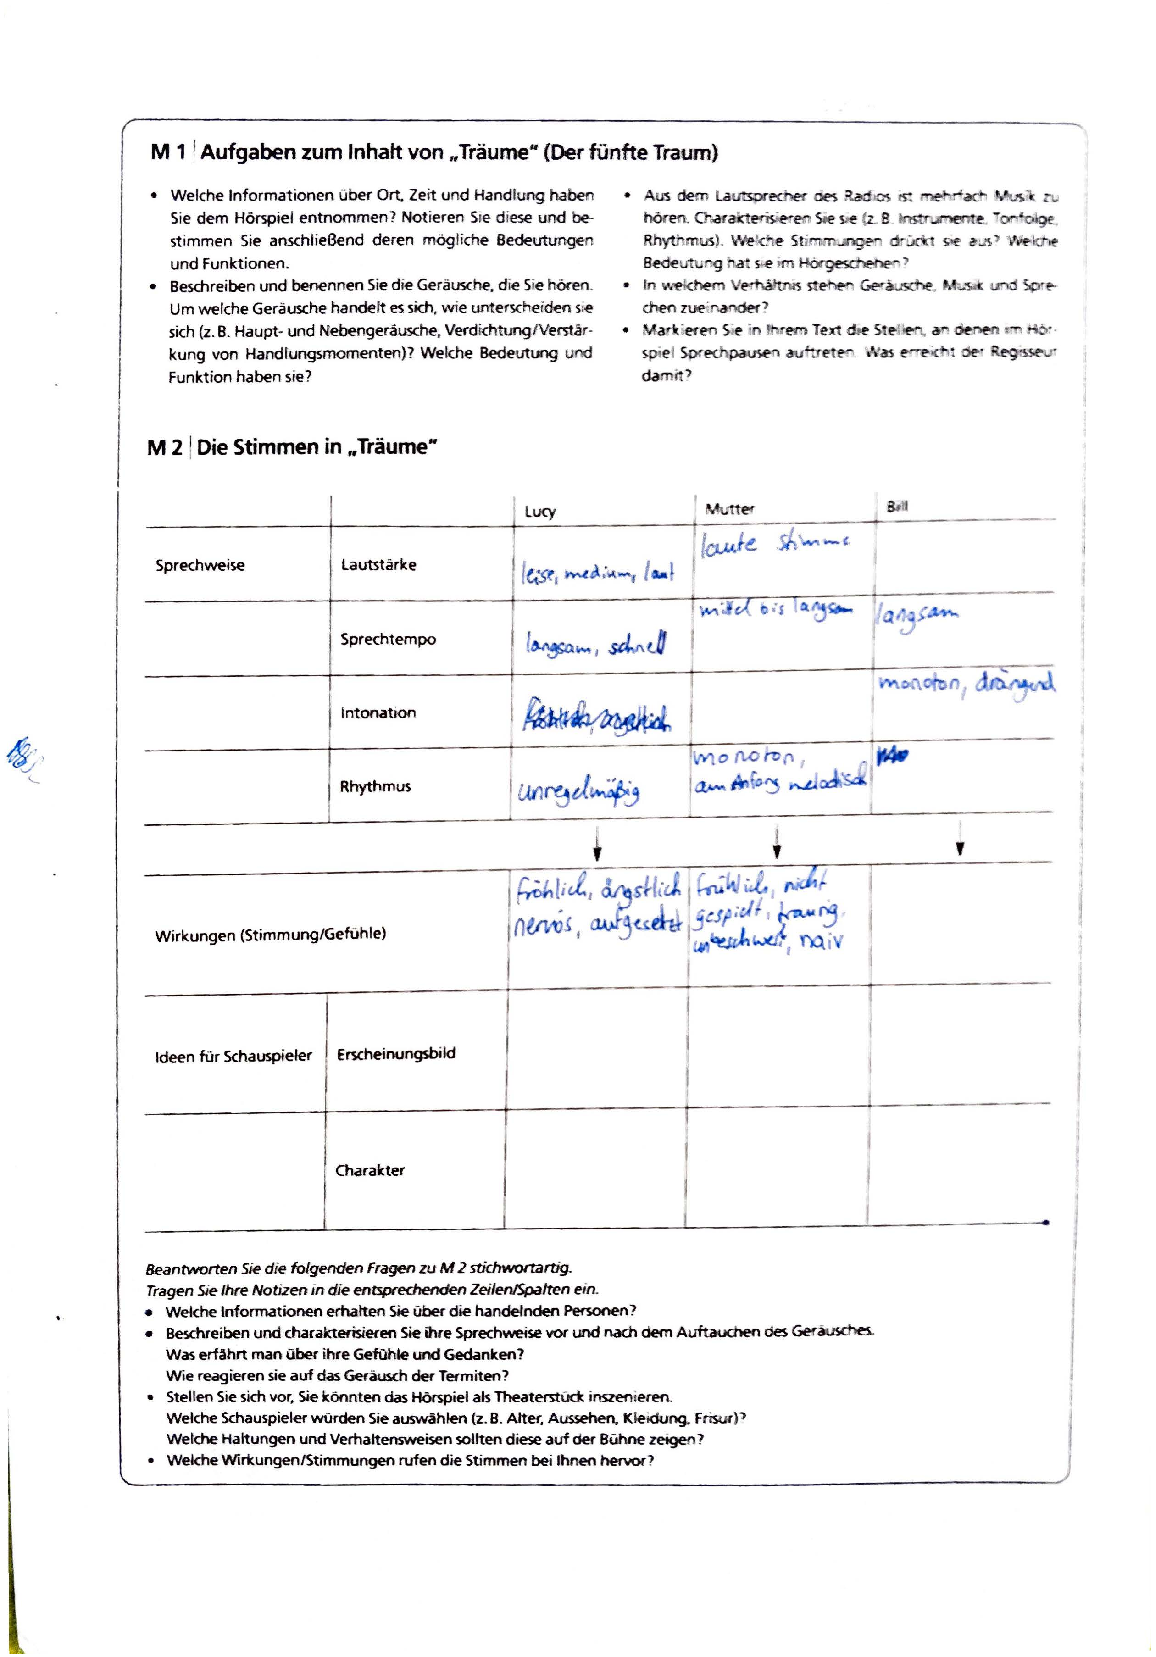
\includepdf[pages=-]{de_inhalt-traume.pdf}
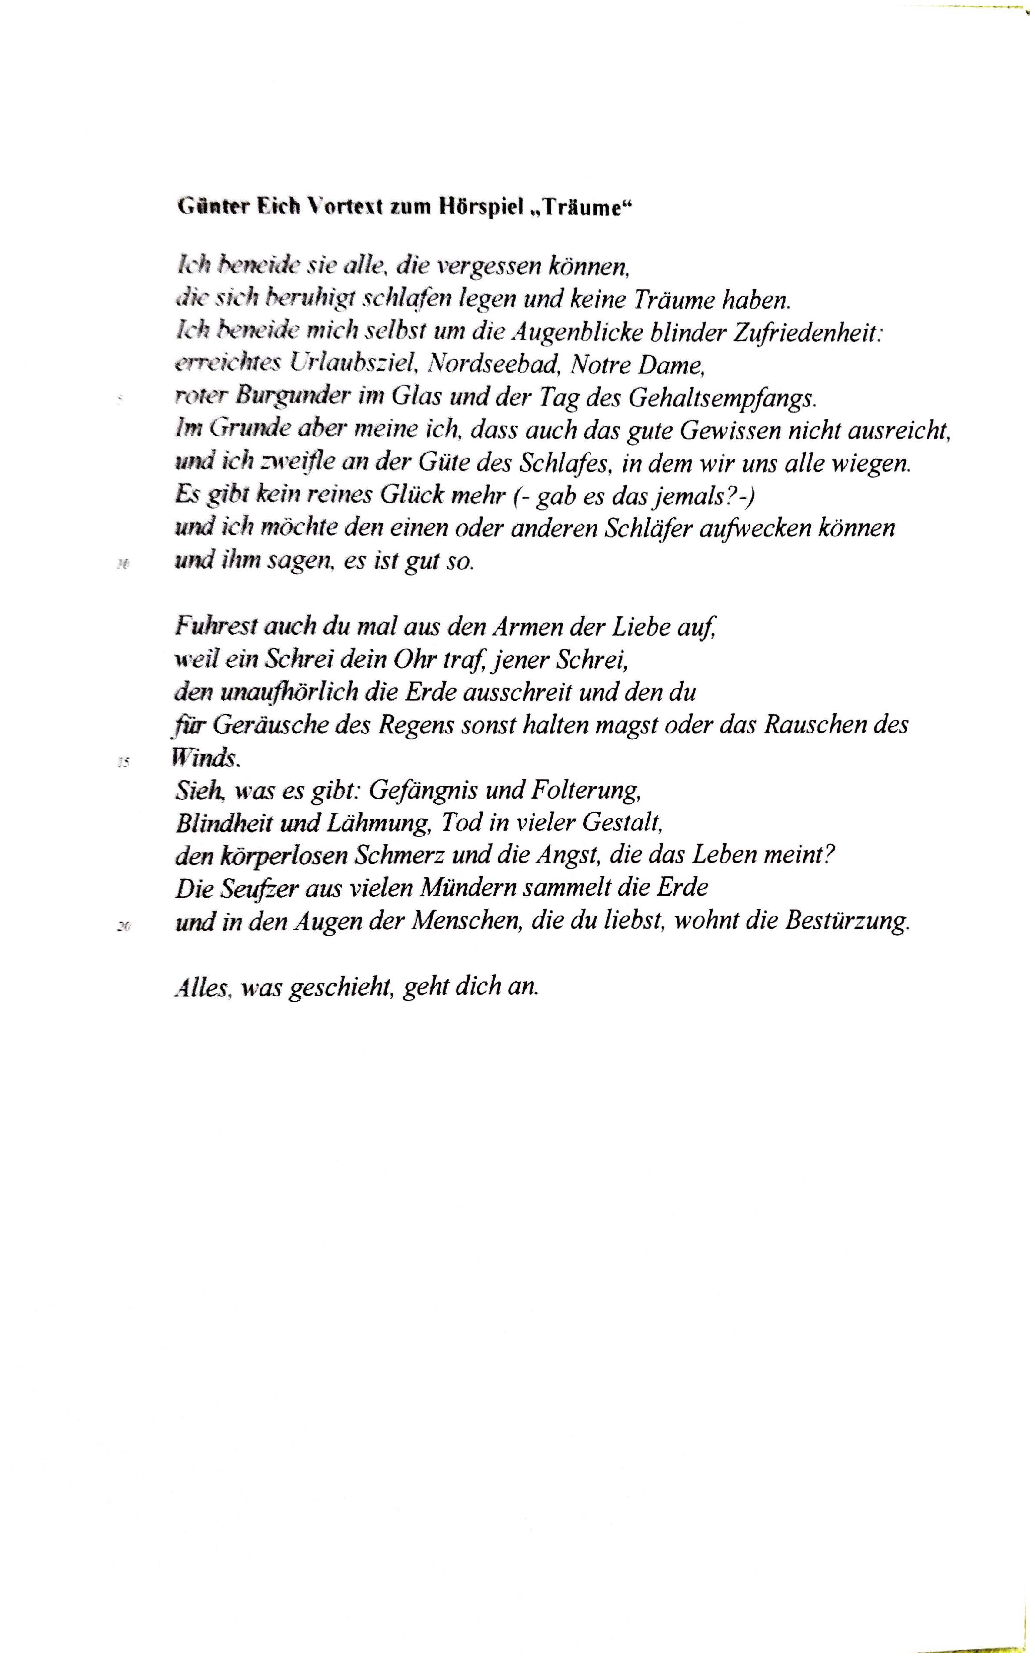
\includepdf[pages=-]{de_traume.pdf}
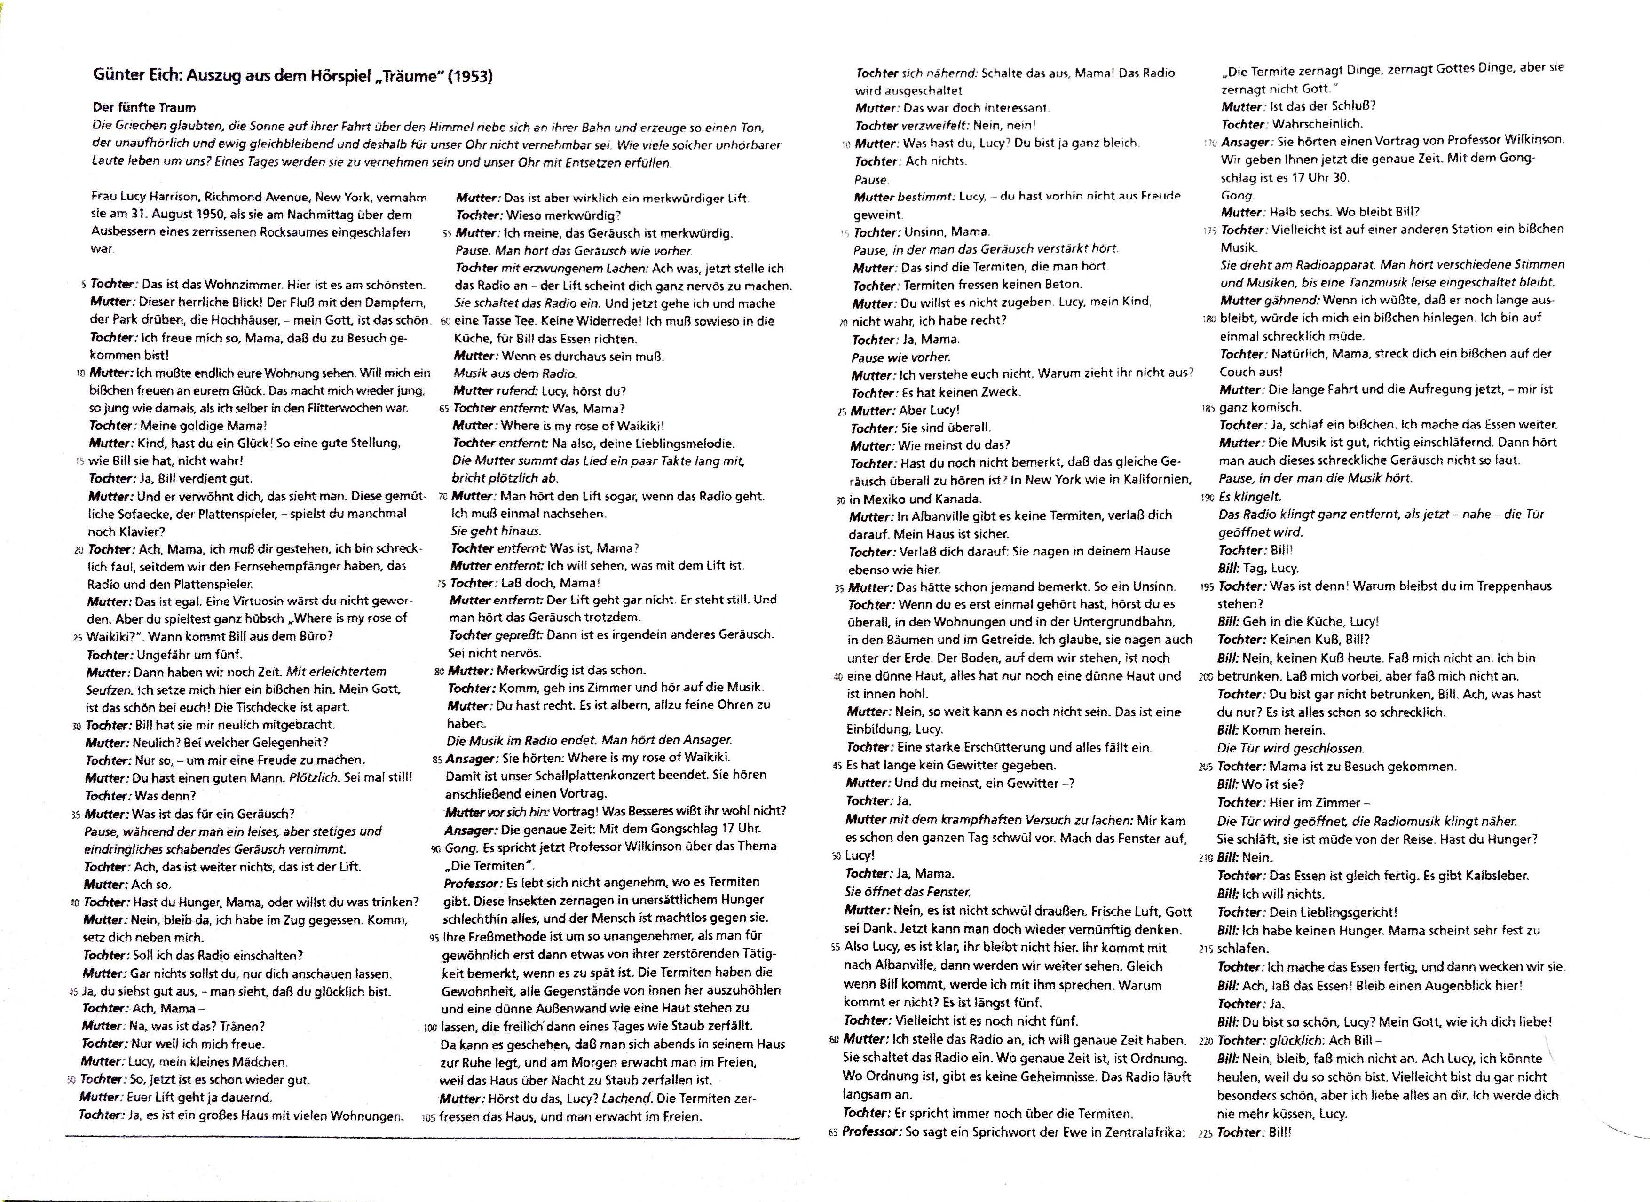
\includepdf[pages=-]{de_traume2.pdf}

\end{document}
